\documentclass[sigplan,screen]{acmart}
\usepackage{pifont}

%
% defining the \BibTeX command - from Oren Patashnik's original BibTeX documentation.
\def\BibTeX{{\rm B\kern-.05em{\sc i\kern-.025em b}\kern-.08emT\kern-.1667em\lower.7ex\hbox{E}\kern-.125emX}}

%
% end of the preamble, start of the body of the document source.

\usepackage[small,compact]{titlesec}
\titlespacing{\section}{0pt}{3pt}{3pt}
\titlespacing{\subsection}{0pt}{2pt}{2pt}
\titlespacing{\subsubsection}{0pt}{1pt}{1pt}

\hypersetup{draft}

\begin{document}

\settopmatter{printacmref=false} % removes citation information below abstract
\renewcommand\footnotetextcopyrightpermission[1]{} % removes footnote with conference information in first column
\pagestyle{plain} % removes running headers
\setcopyright{none} % removes copyright information
%
% The "title" command has an optional parameter, allowing the author to define a "short title" to be used in page headers.
\title{I Know What Was Hacked Last Summer: Auditing Unpopular Kernel Paths for Better Container Security}

%\author{Yiwen Li}
%\affiliation{\institution{New York University}}
%\email{liyiwen@nyu.edu}

%\author{Brendan Dolan-Gavitt}
%\affiliation{\institution{New York University}}
%\email{brendandg@nyu.edu}

%\author{Justin Cappos}
%\affiliation{\institution{New York University}}
%\email{jcappos@nyu.edu}

\maketitle

\section*{Abstract}
One reason why containers, such as Docker and LinuxKit, are so widely used is because of the perceived isolation and security they provide against 
the potentially malicious or buggy user programs running inside of them. Yet, most security measures designed for containers do not take into account 
how to protect against the zero-day kernel bugs inside the kernel itself. 
Containers are vulnerable to these bugs because they allow access to rarely executed paths where such vulnerabilities can be found. 
Limiting kernel access to only frequently used \textbf{\textit{popular paths}}, which have previously been proven to contain fewer security bugs, 
would greatly reduce the risk of triggering these vulnerabilities. 

In this paper, we present a multi-step methodology for improving container security by leveraging data about popular paths into a kernel tailoring strategy. 
It starts with a systematic approach to identifying and capturing the popular paths data for widely-used container applications. 
By evaluating this data at different levels of granularity (line, function, and file), users can get fresh insights into which parts of the kernel are being used, 
and so make informed decisions about which code is safe to execute. 
The data also guided the implementation of a tailored kernel called the \textbf{\textit{UnPopular Action Kernel (UnPAK)}}. 
\textbf{UnPAK} registers when a potentially risky path is reached and can respond with a number of actions, from issuing warning messages to denying execution of commands. 
When testing containers using UnPAK, we found that they were able to run their default workload using just the popular paths more than 99.9\% of the time. 
Furthermore, the kernel was able to operate with only minor increments (0.1\% on average) in runtime overhead, and only around 0.37\% extra cost in memory space. 
Most importantly, since only 6\% of 50 Linux kernel CVE security vulnerabilities we examined were present in the popular paths, 
utilizing the UnPAK system offers a way to reduce the risk of triggering bugs without sacrificing operational efficiency. 
Lastly, UnPAK compares favorably with three other current kernel tailoring strategies, as it is more adaptable to a wider variety of applications, and can reduce the largest amount of attack surface. 
\section{Introduction}
\label{sec.introduction}
Containers continue to grow in popularity, with one industry survey suggesting the technology could become a \$2.7 billion market by 2020 \cite{451-Research}. 
This widespread adoption of containers, such as Docker \cite{Docker} and LinuxKit \cite{LinuxKit}, can be attributed to several factors, 
including portability and elimination of the need for a separate operating system \cite{what-containers-do}.
In addition, the perceived isolation and security they provide to the programs running inside of them is reassuring to users looking to protect their data and operations. 
However, several recent incidents in which zero-day kernel bugs have been triggered from inside of a container \cite{containers-kernel-bug-tcp, containers-runc-vulnerability} 
suggest this perception may not be completely true. 
Furthermore, since the kernel is the critical and privileged code shared by containers and the host system, exploitation of such bugs could lead to severe security problems, 
such as privilege escalation. 
The famous ``Dirty COW'' vulnerability that emerged in 2016, reported as CVE-2016-5195, allowed attackers to escape from a Docker container and access files 
on the host system \cite{dirty-cow}. 
This vulnerability affected all of the Linux-based operating systems that used older versions of the Linux kernel, including Android. 
One analysis, conducted a year after it was first reported, found the bug was being exploited in more than 1200 malicious Android apps, affecting users in at least 40 countries \cite{dirty-cow-impact}. 

The fundamental reason such exploits can occur is that existing containers are designed to directly access the underlying host operating system kernel on which they are run. 
This design makes containers more efficient and lightweight to use—features that make them so attractive to end-users. 
Unfortunately, this access also exposes containers to zero-day bugs within the kernel itself \cite{containers-kernel-bug-tcp}. And, with one OS kernel servicing a number of containers, 
it is common for its code to become bloated, a risk to both security and efficiency. 
While a number of research initiatives have looked at code debloating \cite{DBLP:conf/ccs/GhaffariniaH19, Debloating-Software, RAZOR, Kernel-Debloating}, 
most of these efforts are not broadly applicable, and perform inconsistently, 
Furthermore, they do not eliminate bloat at the line of code level, nor can these approaches broadly identify which parts of the kernel are less likely to host zero day bugs. 
To improve security, the issue is not just reducing the total amount of code, but figuring out which parts of the kernel should be targeted in such a reduction. 

Over the years, several  researchers \cite{Chou, Ozment} have proposed metrics that point to where buggy code might be within the kernel, 
and these strategies have provided some useful  design guidance. 
One such study \cite{Lock-in-Pop}, released three years ago, suggested a powerful correlation between kernel lines accessed by widely-used programs and their likelihood to contain security flaws. 
Furthermore, the study \cite{Lock-in-Pop} demonstrated that these frequently used kernel paths can be leveraged to design and construct secure virtualization systems. 
Building on these results, we ask the question, can we apply the popular paths metric to  securing existing containers? 

In this paper, we study the feasibility of using the popular paths metric to secure the LinuxKit container toolkit. 
The study required a number of steps, starting with finding a  systematic way to gather data on popular paths, 
and affirming that this data is representative of hundreds of widely-used containers from Docker Hub \cite{DockerHub}. 
By analyzing this data at three different levels of granularity—file, function, and lines of code—we found that 
each can provide data values that collectively form a hierarchy of security options from which users can choose, 
based on the security sensitivity of the application. A user can choose to simply analyze the data at the file level to quickly eliminate a significant portion of all security risks, 
or use data gathered at the lines of code level to obtain a broader picture of where bugs are located, and how to avoid them.

Using the raw popular paths data, we were also able to design the \textbf{\textit{UnPopular Action Kernel (UnPAK)}}, 
a modified version of the Linux kernel which is tailored to register any attempt to access infrequently used paths. 
Developing and testing UnPAK contributed to our study in two ways. 
Firstly, it provided usable data on how often applications accessed risky paths, so we could determine how essential such access is for their functionality. 
And, secondly, it offered a chance to program a number of responses into the operations of the kernel, such as a warning system. 
While initially UnPAK  was instrumented to warn users of potentially dangerous behaviors so they can make informed decisions on whether or not to execute it, 
it could also be programmed for other actions, such as automatically refusing such an execution.

When tested at all three of the granularity levels mentioned above, we confirmed that UnPAK can effectively prevent most kernel bugs from being triggered when running Docker containers. 
Only three of the 50 CVE kernel vulnerabilities checked for were found in those LinuxKit paths. 
Even at the file level, our tests showed that security can be improved by simply removing unloaded / unused drivers, and unused architectures, 
as more than half of the kernel bugs reside in these files. 
Better still, an evaluation of our findings affirmed that frequently used Docker containers experience no loss of functionality when using just the popular paths. 
Indeed, we found these paths were used more than 99.9\% of the time to run the official Docker containers' default workload. 
In addition, UnPAK compared favorably as a debloating strategy when run against instantiations of three current kernel tailoring strategies \cite{SALAD18, NDSS13, Linux-Kernel-Tailoring-Framework}. 
It reduced the largest amount of attack surface while offering similar runtime performance. 
UnPAK also offers more flexibility, as many of the existing strategies are tied to a specific application, or to addressing a particular subset of bugs.

Lastly, in our performance evaluation, we found that running UnPAK as currently designed only incurred about 1\% of runtime overhead, 
while the memory space overhead was only about 0.37\%. 
Thus, reduced exposure to bugs could be achieved with very little perceived difference in operation efficiency or cost.

In summary, we make the following contributions in this paper:
\begin{itemize}
	\item We develop a methodology to systematically identify and capture the ``popular paths'' data for widely-used container applications, and verify that the technique works for the most downloaded Docker containers run inside of the LinuxKit VM.  
	\item We evaluate popular paths data at different levels of granularity (line, function, and file) and find that, at each level, following the popular paths metric can provide opportunities to identify and eliminate kernel vulnerabilities.
	\item We use the popular paths data to design and implement UnPAK, a modified version of the Linux kernel. This instrumented kernel logs attempts to trigger unpopular paths and can respond with a number of defensive actions, from sending warning messages to denying execution of the program.
	\item We demonstrate that frequently-used Docker containers were able to run their default workload using the popular paths more than 99.9\% of the time, with only a negligible (less than 1\%) performance overhead. 
	\item We compare the UnPAK strategy to three other kernel tailoring approaches and find that, as currently configured, it can reduce the largest amount of attack surface, and is more adaptable to a wider variety of applications.
\end{itemize}
\section{Background and Motivation}
\label{sec.motivation}
The concept of OS virtualization, where an operating system runs programs in an isolated space over a kernel, has been around for several decades \cite{OS-Level-Virtualization}. 
Yet,  the emergence of container programs \cite{Containers_and_VirtualMachines}, which run off the kernel's OS and therefore have a lower overhead, 
has spurred  growth in the popularity of these machines, as  Docker \cite{Docker}, LinuxKit \cite{LinuxKit}, and Kubernetes \cite{Kubernetes}, have seen wider adoption over the past few years. 
For example, Docker Hub \cite{DockerHub} holds more than two million container images , and the most popular ones have been downloaded by more than ten million users. 
Many users prefer using containers over traditional full-scale virtual machines such as VMware workstation \cite{VMWare-Workstation} and VirtualBox \cite{VirtualBox}, 
because containers allow them to test and develop their software programs with relatively low overhead. 
In addition, the idea of running their programs in a ``contained'' environment tends to make developers feel they have secured them against all threats. 

Existing container systems use several mechanisms to provide isolation and security to the programs running inside of them. 
Namespaces [8] were a modern Linux kernel feature, introduced between Linux kernel version 2.6.15 and 2.6.26, to provide a global system resource abstraction 
that helps achieve isolation between different containers. Docker and LXC [9] containers also used namespaces to provide isolation. 
Control groups [10] are another key Linux feature that enables accounting and limiting important system resources, such as memory, CPU, and disk I/O, to each container.  
In addition, this feature helps prevent denial-of-service attacks. Linux kernel capabilities [11] are used by a number of container systems, including Docker. 
Capabilities allow containers restrict permissions on specific resources, such as network and file system. 
Modern Linux kernels also have other kernel hardening systems, such as AppArmor [12], SELinux [13], GRSEC [14], PAX [15], etc., 
that may be leveraged by containers to provide some extra safety. GRSEC and PAX add safety checks at compile-time and run-time of the kernel. 
Docker ships a template that works with AppArmor, and also has SELinux policies working with Red Hat [16]. 
These kernel hardening systems are mostly access control mechanism that provides safety in the similar way that capabilities do.

While containers leverage existing mechanisms to try to improve security, there is yet one fundamental issue that is really challenging to address. 
The problem is, as acknowledged above,  that unlike ia full-scale virtual machine, the operating system kernel is shared among all containers and the host. 
This magnifies the damage a kernel vulnerability could cause. If a bug in the kernel was triggered from one guest container, it could result in a security problem for other containers, 
and even the host, breaking all the isolation that users expect to get from a container.

The threat of zero-day kernel vulnerabilities is the main motivation behind this work. 
This research initiative was launched to prevent zero-day kernel bugs from being triggered in containers, while still allowing containers to perform their desired workload. 
Having already established in a previous paper that   implementing the popular paths metric i could identify and neutralize the threat of these bugs [3] 
we theorized that container security can be enhanced in the same manner. 
To prove this hypothesis, we created a new design implementation for container security that is described in detail in the following section.
\section{Design and Implementation}
\label{sec.design}

Designing an implementation of the popular paths metric for use with containers required completion of two separate tasks. 
First, we had to find the popular paths for the underlying host operating system. 
And, second, once we knew where these paths were, we needed a way to log / block the unpopular paths to warn and keep containers away from these less-used and potentially buggy code paths. 
Our solution was a dual module approach we call the Secure Logging System (Shown in Figure \ref{fig:design}). 

\subsection{Design of Our ``Secure Logging System''}
\label{sec.design.secure_logging_system}
Identifying the popular paths for the given container system is handled by the system module we refer to as the Kernel Profiler. 
This module identifies the lines of code in the host kernel that are executed when running its default / regular workload. 
Such a workload is often defined in the configuration files (Dockerfiles) that come with the container images. 
We collected  ``popular paths kernel traces,'' as we named them, from a set of the containers, as  ranked ``most popular'' by the number of user downloads. 

\begin{figure*}
\centering
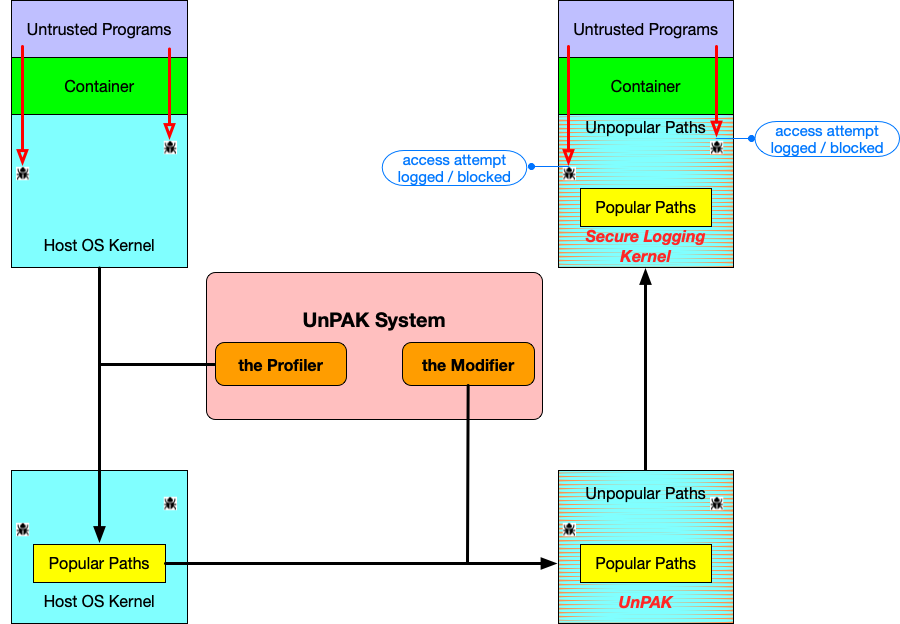
\includegraphics[width=1.5\columnwidth]{diagram/design.png}
\caption{\small Design overview of our Secure Logging System}
\label{fig:design}
\end{figure*}

In effect, the Profiler sets out a map highlighting places in the kernel that are safe for an application to access. 
The second module, the Kernel Modifier,  uses this map to instrument the rarely used unpopular paths to either generate security warning messages / logs, or to block code execution on these paths. 
When both modules are implemented, the result is an instrumented Linux kernel with security monitors and checks inserted at the non-popular paths. 
This Secure Logging Kernel can then be used to run containers without any required changes to the containers themselves.

\subsection{Implementation}
\label{sec.design.implementation}
To adapt our design for real-world containers  and applications, it was necessary to build our own infrastructure. This section describes in detail how the modules in our system were implemented.

\subsubsection{Implementing the Kernel Profiler}
\label{sec.design.implementation.kernel_profiler}
The Kernel Profiler is designed to collect the kernel trace of running user containers. 
The popular paths kernel trace we are looking to identify refers to the lines of code in the underlying host operating system kernel that were executed when running the regular container workload. 
This workload is defined in the configuration files of the corresponding images from containers we labeled popular based on the number of user downloads. 
Our Kernel Profiler works in the following way: 
\begin{enumerate}
	\item The Linux kernel used to run the Docker containers is recompiled with the Gcov \cite{gcov} kernel profiling feature enabled. 
	\item To run the Docker containers, the Kernel Profiler first automatically generates the configuration file for the Gcov-enabled LinuxKit. 
	This file will define the task container, along with a data container responsible for collecting, storing, and transferring the kernel trace data. 
	\item When booting the LinuxKit virtual machine, a script in the profiler automatically starts running the workload of the task container. 
	The profiler will collect the kernel trace data, in the form of gcda files generated by Gcov, store them at ``/sys/kernel/debug/gcov/,'' 
	and by the end of the run transfer the data to the host system for further use. 
	\item Using the lcov \cite{lcov} tool to process the kernel trace data collected from the host system, the profiler generates formatted data about which lines of code were executed in the kernel source files. 
	These files will be used by the  Kernel Modifier to identify the unpopular paths that must trigger an alert if used. 
\end{enumerate}

\begin{figure*}
\centering
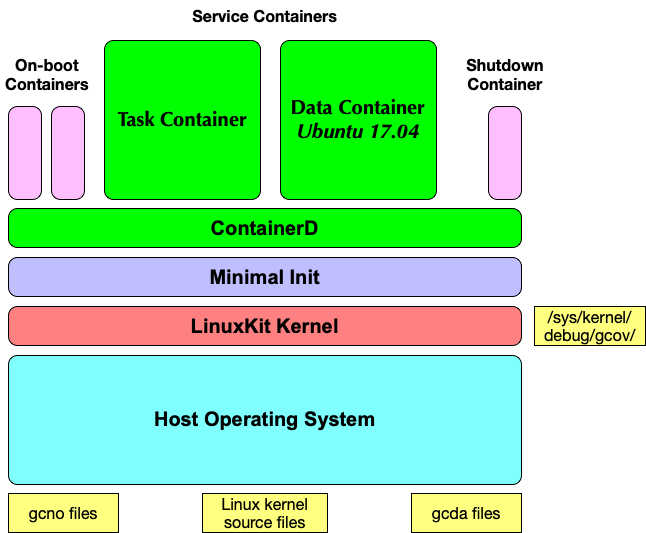
\includegraphics[width=1.5\columnwidth]{diagram/linuxkit-kernel-profiler.png}
\caption{\small Implementation of the Kernel Profiler}
\label{fig:linuxkit-kernel-profiler}
\end{figure*}

\subsubsection{Implementing the Kernel Modifier}
\label{sec.design.implementation.kernel_modifier}
For the Kernel Modifier to insert security logging code at the unpopular paths in the Linux kernel, It needs to first identify the correct places in the kernel source files to be instrumented. 
It can then modify the code as needed. The Kernel Modifier has three main parts: the Clang compiler, the Clang analyzer, and the kernel instrumenting tool (Shown in Figure \ref{fig:linuxkit-kernel-modifier}).
It operates in the following way: 
\begin{enumerate}
	\item The Clang C compiler from the Clang / LLVM project \cite{llvm}, along with a BEAR \cite{bear} tool compiled the Linux kernel source. Using BEAR, 
	we can generate a compilation database containing all the compile flags and options needed for the process. 
	In turn, this database will be used by our Clang analyzer to perform source code parsing in the next step.
	\item Once we have the compilation database for the Linux kernel,  we use the Clang analyzer to perform static analysis on the kernel source code to obtain the control flow graph for each function in the files. 
	The analyzer leveraged Clang’s LibTooling \cite{clang-libtooling} to construct the AST tree from the kernel source code, and then obtain the control flow graph. 
	With this graph, we can identify the corresponding source line number for each basic block. Furthermore, the beginning lines of all the blocks in the source files are candidates for places to add security logging code. 
	Here, a basic block refers to a straight-line code sequence with no branches in except to the entry and no branches out except at the exit. 
	Thus, if a basic block is unpopular, it is sufficient to insert only one piece of secure logging code at the beginning of it to monitor and warn the attempt to reach that code. 
	This approach can optimize our instrumentation by  avoiding redundancy in our code injection.  
	\item The next steps has the kernel instrumenting tool executing modifications based on both the basic blocks, and the collected popular paths data . 
	The algorithm for our kernel modification directs us through the basic blocks in the kernel source files. If none of the lines in a block are in the popular paths data, we consider this an unpopular basic block, 
	and our instrumenting tool will add the security logging code at the beginning of this block. If we discover that an entire function has no  lines in the popular paths data, we consider this an unpopular function, 
	and just add our security logging code once where it starts . This allows us to avoid adding redundant and unnecessary code. 
	The secure logging code we inserted in front of the unpopular paths was a kvm hypercall from the LinuxKit kernel into the host Linux kernel (Shown in Figure \ref{fig:kvm_hypercall}). 
	In this way, we can guarantee minimal affect on the LinuxKit kernel functionality, while still being able to generate security logging whenever unpopular paths were reached.
	\item Our Kernel Modifier automatically inserts our secure logging code at beginning of the unpopular paths in the Linux kernel source files, 
	and then recompiles the kernel to produce the Secure Logging Kernel, which can be directly used to run Docker containers in the LinuxKit VM. 
\end{enumerate}

\begin{figure*}
\centering
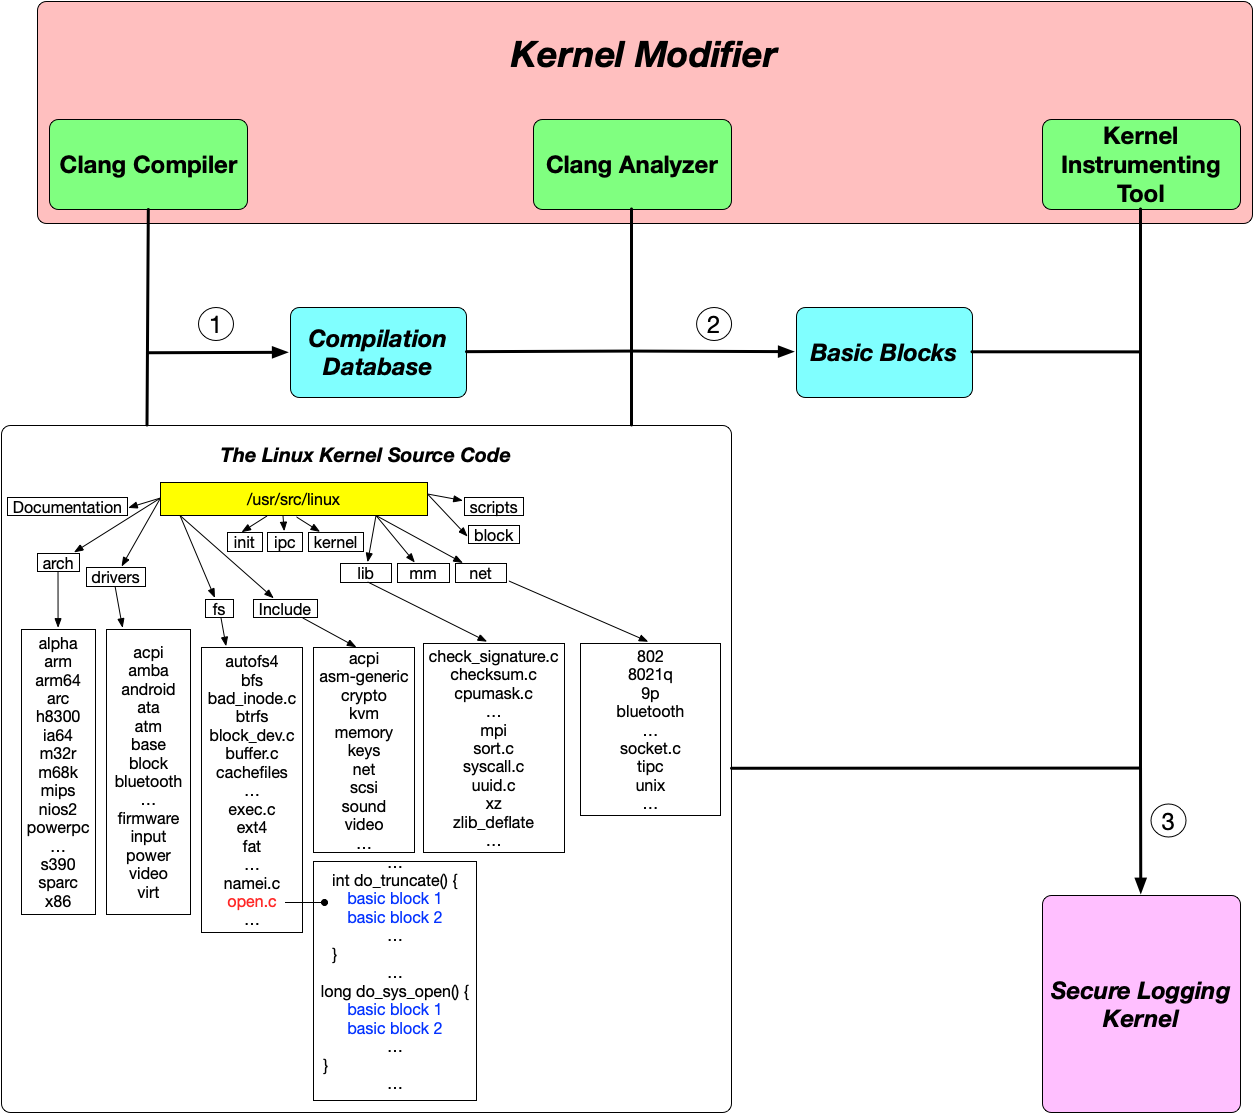
\includegraphics[width=1.5\columnwidth]{diagram/linuxkit-kernel-modifier.png}
\caption{\small Implementation of the Kernel Modifier}
\label{fig:linuxkit-kernel-modifier}
\end{figure*}

\begin{figure*}
\centering
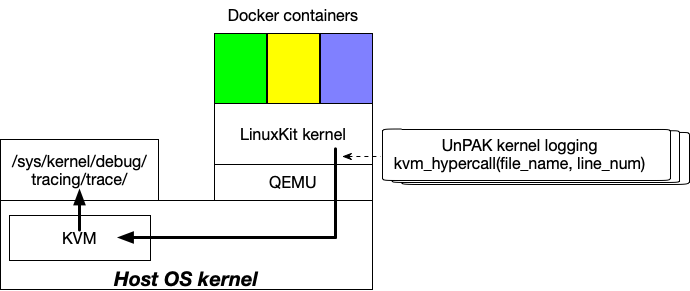
\includegraphics[width=1.5\columnwidth]{diagram/kvm_hypercall.png}
\caption{\small Our KVM\_HYPERCALL kernel instrumentation}
\label{fig:kvm_hypercall}
\end{figure*}

\section{Evaluation}
\label{sec.evaluation}
To demonstrate that our proposed solution for container forensic auditing with UnPAK and SmashPAK is practical and efficient, 
we conducted a series of tests to answer the following questions: 
\begin{itemize}
	\item Can we build the popular paths kernel profile for containers in a systematic way? (Section~{\ref{sec.evaluation.1}})
	\item Can an analysis of the popular paths data for containers help developers and researchers perform efficient security auditing? (Section~{\ref{sec.evaluation.2}})
	\item Can real-world containers run on the UnPAK auditing kernel with no loss of functionality? (Section~{\ref{sec.evaluation.3}})
	\item What is the performance overhead of using UnPAK to audit, as opposed to using the original Linux kernel? (Section~{\ref{sec.evaluation.4}})
	\item Is forensic auditing using SmashPAK efficient? (Section~{\ref{sec.evaluation.5}})
\end{itemize}

\subsection{Can popular paths kernel profiles for containers be built in a systematic way?}
\label{sec.evaluation.1} 
Our UnPAK auditing kernel relies on the popular paths data to locate the places where auditing is likely to reveal a previous bug exploit. 
Having a systematic way to build the popular paths kernel profile for containers is key to making its use scalable, reproducible, and accessible to developers and the research community. 
Therefore, the first step in our investigation was developing and testing such a standard procedure for containers. 
This procedure can be divided into three stages: selecting the \textbf{dataset}, assembling \textbf{a profiling framework}, and conducting the \textbf{experiment}. 

\textbf{The dataset:} The dataset stage involved selecting the containers to use and the workload that would run inside of  them. 
We wanted the defined dataset to be representative of the containers used by millions of clients, so we sourced a set accepted as widely used according to trustworthy real-world statistics.  
We selected 50 containers deemed most popular on Docker Hub according to their official number of pulls. Each selected container had more than 10 million pulls \cite{DockerHub}. 
The workload run by each was the set of commands or operations defined in the official Dockerfile ``CMD'' section for each container image.

\textbf{The profiling framework:} This next stage involved establishing a running environment and capturing the actual data, a procedure that required a robust framework. 
Ideally we wanted the framework to be portable so it could be used across different platforms. 
We selected the LinuxKit VM, which works with Linux, Windows, and Mac OS, and a Linux kernel with a Gcov profiling tool enabled to run the Docker containers. 
This framework works with  other Linux kernel versions, which makes the procedure more widely applicable. 

\textbf{The experiment:}  The test itself consisted of running the containers with their defined workloads in the profiling framework, and extracting the resulting  data. 
The procedure was able to automate the experimental runs in a way that allowed users to define key variables of the input, including the exact version of the container image to use, 
and the number of iterations to run for each container. By making  these design choices flexible, 
it was better able to accommodate container application users and developers with different needs and computing resources. In our experiment, 
we decided to do 10 iterations, because it provides a sufficient number of runs to make the data reliable, without consuming too much time and computing resources. 
In our experiment, we were able to automatically collect the popular paths data based on a training dataset of 50 popular Docker containers to build our kernel profile, 
which was then used to produce our UnPAK auditing kernel. 

\subsection{Can the popular paths data for containers help developers and researchers perform efficient security auditing?}
\label{sec.evaluation.2} 
Using the procedures described above, we obtained data for some of the most frequently accessed  containers on Docker Hub, and used it to check for security vulnerabilities. 
We started with a list of all 50 of the CVE kernel vulnerabilities for Linux kernel version 4.14.x that were available from the National Vulnerability Database when our study 
was conducted (July 2019) \cite{NVD} and identified the kernel patch that fixed the bug. 
This allowed us to identify the source line numbers, functions and files that corresponded to it, and use this information to highlight where these bugs were located in the kernel.   

It should be noted that 49 out of the 50 bugs tested in this experiment were discovered and confirmed \textit{after} publication of the original popular paths study \cite{Lock-in-Pop}. 
This shows that the metric can indeed effectively predict where bugs are likely to occur, and thus provide a solid basis for guiding efficient kernel auditing.  

The raw data generated by Gcov in the profiling framework was at the line-of-code level, as this is the level at which  the initial popular path study \cite{Lock-in-Pop} was performed. 
We wanted, however, to generate  additional information at the function and file level. 
Having these three different levels of granularity provides a full map of how the kernel code was used by containers and where the vulnerabilities might lie in each.

In the discussion below, we label files and functions with four different categories based on the popularity data. 
Those labeled ``unpop'': contain 0 lines of popular code; ``all-pop'': contain 100\% popular code lines; ``partial-pop'': contain at least 1 line of popular code 
and 1 line of unpopular code. ``Pop'' is the combined lines of all-pop + partial-pop.

\textbf{Popular paths data at the file level}
\newline
For developers and security teams, the first thing to identify is which files are popular, as this can be a first step to secure the kernel without needing to 
deal with the complex logic and branches inside of each file. 

From our data (shown in Table \ref{tab:cve_files})), we can see that the ``all-pop'' files contain no bugs  and thus are the safest ones to use.  
Alternatively, the  ``unpop'' files contain more than half of the bugs. The higher bug density of the unpopular files suggests that removing these files could be an easy first step to securing the kernel. 

 ``Partial-pop'' files, which accounted for about 30\% of the bugs investigated, present a trickier problem to resolve. 
 The presence of some popular lines means these items are being used and can not simply be removed. If stricter security requirements are desired, 
 we need to go inside of these files to look at a finer granularity, which is the function level. 
 
\begin{table}
\small
\caption{CVE bugs located in Unpopular and Popular kernel files}
\label{tab:cve_files}
\begin{tabular}{l|r|r|r|r|r}
 kernel & unpop & pop & all-pop & partial-pop & total \\
 dir & \color{red}{(CVEs)} & \color{red}{(CVEs)} & \color{red}{(CVEs)} & \color{red}{(CVEs)} & \\
 \hline
 arch & 133\color{red}{(3)} & 272\color{red}{(1)} & 81 & 191\color{red}{(1)} & 405 \\
 \hline
 block & 10 & 44 & 0 & 44 & 54 \\
 \hline
 crypto & 53\color{red}{(1)} & 89\color{red}{(2)} & 0 & 89\color{red}{(2)} & 142 \\
 \hline
 drivers & 161\color{red}{(11)} & 543\color{red}{(3)} & 5 & 538\color{red}{(3)} & 704 \\
 \hline
 fs & 52\color{red}{(6)} & 176\color{red}{(2)} & 5 & 171\color{red}{(2)} & 228 \\
 \hline
 ipc & 1 & 9 & 0 & 9 & 10 \\
 \hline
 kernel & 40\color{red}{(2)} & 183 & 2 & 181 & 223 \\
 \hline
 mm & 16\color{red}{(1)} & 59\color{red}{(4)} & 0 & 59\color{red}{(4)} & 75 \\
 \hline
 net & 266\color{red}{(5)} & 482\color{red}{(3)} & 0 & 482\color{red}{(3)} & 748 \\
 \hline
 security & 6 & 17 & 0 & 17 & 23 \\
 \hline
 total & 738\color{red}{(29)} & 1874\color{red}{(15)} & 93 & 1781\color{red}{(15)} & 2612 \\
 \hline 
 percent & 28.3\% & 71.7\% & 3.6\% & 68.1\% & 100\% \\
 & \color{red}{(66\%)} & \color{red}{(34\%)} & \color{red}{(0\%)} & \color{red}{(34\%)} &
\end{tabular}
\textit{\textbf{unpop}: contain 0 line of popular code.} \\
\textit{\textbf{all-pop}: every line is popular code.} \\
\textit{\textbf{partial-pop}: contain at least 1 line of popular code and 1 line of unpopular code.} \\
\textit{\textbf{pop}: all-pop + partial-pop.}
\end{table}

\textbf{Popular paths data at the function level}
\newline
Using the raw data, shown in Table \ref{tab:cve_functions}, we pinpoint which functions were used by popular containers. 
Our data shows that ``unpop'' functions contain 5x more bugs than ``pop'' functions, while the ``all-pop'' functions contain only one bug. 

As with the file analysis above, having this information can help security teams eliminate some risks by just avoiding the less-used functions. 
Unfortunately, that still leaves the ``partial-pop'' functions, which  contain 12 bugs.  As with the ``partial-pop'' files, 
the presence of some frequently used functions in this group means they cannot  simply be removed at this level. 
While analyzing each function at the line-of-code level is the most labor intensive of the methods elaborated here, it offers the best opportunity to remove risky code. 
Below we look at vulnerabilities revealed by the popular paths data at this most fine-grained level. 

\begin{table}
\small
\caption{CVE bugs located in Unpopular and Popular kernel functions}
\label{tab:cve_functions}
\begin{tabular}{l|r|r|r|r|r}
 kernel & unpop & pop & all-pop & partial-pop & total \\
 dir & \color{red}{(CVEs)} & \color{red}{(CVEs)} & \color{red}{(CVEs)} & \color{red}{(CVEs)} & \\
 \hline
 arch & 1528\color{red}{(7)} & 968\color{red}{(1)} & 312 & 656\color{red}{(1)} & 2496 \\
 \hline
 block & 777 & 264 & 68 & 196 & 1041 \\
 \hline
 crypto & 527\color{red}{(6)} & 121 & 36 & 85 & 648 \\
 \hline
 drivers & 6258\color{red}{(20)} & 2640 & 562 & 2078 & 8898 \\
 \hline
 fs & 1888\color{red}{(13)} & 1653\color{red}{(3)} & 559 & 1094\color{red}{(3)} & 3541 \\
 \hline
 ipc & 138 & 102 & 33 & 69 & 240 \\
 \hline
 kernel & 3562\color{red}{(8)} & 2280 & 793 & 1487 & 5842 \\
 \hline
 mm & 976\color{red}{(2)} & 889\color{red}{(6)} & 281 & 608\color{red}{(6)} & 1865 \\
 \hline
 net & 3703\color{red}{(9)} & 2405\color{red}{(3)} & 695\color{red}{(1)} & 1710\color{red}{(2)} & 6108 \\
 \hline
 security & 179 & 201 & 104 & 97 & 380 \\
 \hline
 total & 19536\color{red}{(65)} & 11523\color{red}{(13)} & 3443\color{red}{(1)} & 8080\color{red}{(12)} & 31059 \\
 \hline 
 percent & 62.9\% & 37.1\% & 11.1\% & 26\% & 100\% \\
 & \color{red}{(83.3\%)} & \color{red}{(16.7\%)} & \color{red}{(1.3\%)} & \color{red}{(15.4\%)} &
\end{tabular}
\end{table}

\begin{table*}
  \begin{center}
    \caption{Evaluation of the CVE vulnerabilities at the line level}
    \label{tab:evaluation_cve}
    \begin{tabular}{c|l|c|c|c} % <-- Alignments: 1st column left, 2nd middle and 3rd right, with vertical lines in between
      \textbf{\#} & \textbf{CVE ID} & \textbf{CVSS Score} & \textbf{Description} & \textbf{Detected in the}\\
       & & & & \textbf{LinuxKit Popular Paths}\\
      \hline
      1 & CVE-2019-10124 & 7.8 & denial of service, in mm/memory-failure.c & \ding{55}\\
      2 & CVE-2019-9213 & 4.9 & kernel NULL pointer dereferences, in mm/mmap.c & \ding{55}\\
      3 & CVE-2019-9003 & 7.8 & use-after-free & \ding{55}\\
      4 & CVE-2019-8956 & 7.2 & use-after-free & \ding{55}\\
      5 & CVE-2019-8912 & 7.2 & use-after-free & \ding{55}\\
      6 & CVE-2019-7308 & 7.5 & out-of-bounds speculation on pointer arithmetic & \ding{55}\\
      7 & CVE-2019-3701 & 7.1& privilege escalation & \ding{55}\\
      8 & CVE-2018-1000204 & 6.3 & copy kernel heap pages to the userspace & \ding{55}\\
      9 & CVE-2018-1000200 & 4.9 & NULL pointer dereference & \ding{55}\\
      10 & CVE-2018-1000026 & 6.8 & denial of service & \ding{55}\\
      11 & CVE-2018-20511 & 2.1 & privilege escalation & \ding{55}\\
      12 & CVE-2018-20169 & 7.2 & mishandle size checks & \ding{55}\\
      13 & CVE-2018-18690 & 4.9 & unchecked error condition & \ding{55}\\
      14 & CVE-2018-18445 & 7.2 & out-of-bounds memory access & \ding{55}\\
      15 & CVE-2018-18281 & 4.6 & improperly flush TLB before releasing pages & \ding{55}\\
      16 & CVE-2018-18021 & 3.6 & denial of service & \ding{55}\\
      17 & CVE-2018-16862 & 2.1 & the cleancache subsystem incorrectly clears an inode & \ding{55}\\
      18 & CVE-2018-16658 & 3.6 & local attackers could read kernel memory & \ding{55}\\
      19 & CVE-2018-16276 & 7.2 & privilege escalation & \ding{55}\\
      \color{red}{20} & \color{red}{CVE-2018-15594} & \color{red}{2.1} & \color{red}{spectre-v2 attacks against paravirtual guests} & \color{red}{\ding{51}}\\
      \color{red}{21} & \color{red}{CVE-2018-15572} & \color{red}{2.1} & \color{red}{userspace-userspace spectreRSB attacks} & \color{red}{\ding{51}}\\
      22 & CVE-2018-14646 & 4.9 & NULL pointer dereference & \ding{55}\\
      23 & CVE-2018-14634 & 7.2 & integer overflow, privilege escalation & \ding{55}\\
      24 & CVE-2018-14633 & 8.3 & stack buffer overflow & \ding{55}\\
      25 & CVE-2018-14619 & 7.2 & privilege escalation & \ding{55}\\
      26 & CVE-2018-13406 & 7.2 & integer overflow & \ding{55}\\
      27 & CVE-2018-12904 & 4.4 & privilege escalation & \ding{55}\\
      28 & CVE-2018-11508 & 2.1 & local user could access kernel memory & \ding{55}\\
      29 & CVE-2018-11412 & 4.3 & ext4 incorrectly allows external inodes for inline data & \ding{55}\\
      30 & CVE-2018-10940 & 4.9 & incorrect bounds check allows kernel memory access & \ding{55}\\
      31 & CVE-2018-10881 & 4.9 & denial of service & \ding{55}\\
      32 & CVE-2018-10880 & 7.1 & denial of service & \ding{55}\\
      33 & CVE-2018-10879 & 6.1 & use-after-free & \ding{55}\\
      34 & CVE-2018-10878 & 6.1 & denial of service & \ding{55}\\
      35 & CVE-2018-10074 & 4.9 & denial of service & \ding{55}\\
      36 & CVE-2018-10021 & 4.9 & denial of service & \ding{55}\\
      37 & CVE-2018-8781 & 7.2 & code execution in kernel space & \ding{55}\\
      38 & CVE-2018-6555 & 7.2 & denial of service & \ding{55}\\
      39 & CVE-2018-6554 & 4.9 & denial of service & \ding{55}\\
      40 & CVE-2018-5390 & 7.8 & denial of service & \ding{55}\\
      41 & CVE-2018-1130 & 4.9 & NULL pointer dereference & \ding{55}\\
      \color{red}{42} & \color{red}{CVE-2018-1120} & \color{red}{3.5} & \color{red}{denial of service} & \color{red}{\ding{51}}\\
      43 & CVE-2018-1118 & 2.1 & kernel memory leakage & \ding{55}\\
      44 & CVE-2018-1068 & 7.2 & write to kernel memory & \ding{55}\\
      45 & CVE-2017-1000410 & 5.0 & leaking data in kernel address space & \ding{55}\\
      46 & CVE-2017-1000407 & 6.1 & denial of service & \ding{55}\\
      47 & CVE-2017-1000405 & 6.9 & overwrite read-only huge pages & \ding{55}\\
      48 & CVE-2017-18224 & 1.9 & race condition, denial of service & \ding{55}\\
      49 & CVE-2017-18216 & 2.1 & NULL pointer dereference, denial of service & \ding{55}\\
      50 & CVE-2015-5327 & 4.0 & out-of-bounds memory read & \ding{55}\\
    \end{tabular}
  \end{center}
\end{table*}

\textbf{Popular paths data at the line level}
\newline
An analysis of the gathered data at the line level shows that the popular lines make up about  20\% of the kernel codebase, 
and that only 6\% (or three) of the CVE bugs were detected in those lines (Table \ref{tab:evaluation_cve}.) 
These three bugs were in commonly used kernel code that, to the best of our knowledge, 
cannot be avoided by any existing security systems. We describe these three bugs in more detail below.  

It is important, to note, however, that two of these bugs  (CVE-2018-15594 and CVE-2018-15572) are Spectre-related hardware vulnerabilities, 
based on fundamental flaws in CPU’s data cache and speculative execution. 
These flaws affect many modern processors \cite{ProjectZero}, and software tools and compartmentalization techniques are not designed to prevent them. 
The only software-related bug is  CVE-2018-1120, which is related to the \texttt{mmap()} system call, and regularly accessed by virtualization systems. 

\noindent
\textbf{[CVE-2018-15594]} 
\newline
This bug lies in \texttt{arch/x86/kernel/paravirt.c} in the Linux kernel before 4.18.1. The source code mishandles certain indirect calls, 
making it easier for attackers to conduct Spectre-v2 attacks against paravirtual guests. 
This bug occurs because the code inside of the \texttt{paravirt\_patch\_call()} function in \texttt{arch/x86/kernel/paravirt.c} is used to rewrite an indirect call with a direct call, 
an essential function used to support Linux kernel paravirtualization. 

\noindent
\textbf{[CVE-2018-15572]} 
\newline
The \texttt{spectre\_v2\_select\_mitigation}  \\ 
function in \texttt{arch/x86/kernel/cpu/bugs.c} in the Linux kernel before 4.18.1 does not always fill RSB upon a context switch. 
As this piece of code in \\
\texttt{spectre\_v2\_select\_mitigation(void)} function would be used by every program as the kernel attempts to mitigate potential Spectre attacks, 
it explains why it appeared in the LinuxKit popular paths. 

\noindent
\textbf{[CVE-2018-1120]} 
\newline
This vulnerability was found affecting the Linux kernel before version 4.17. by 
\texttt{mmap()ing} a FUSE-backed file onto the memory of a process containing command line arguments (or environment strings). 
It appears in the popular paths because \texttt{mmap()} is a commonly used system call. 
Furthermore, this vulnerability involves \texttt{proc\_pid\_cmdline\_read()} and \texttt{environ\_read()} functions that are commonly invoked by virtual machines and user programs. 

The fact that 94\% of bugs were located in the unpopular paths demonstrates that monitoring the unpopular paths to target kernel auditing is a correct choice, 
as an UnPAK kernel based on data above would be able to catch the overwhelming majority of bugs. In addition, the 6\% of bugs missed were in the popular paths, 
and are used by almost every program during their normal runs, which means that they were quite easy to catch and thus far less interesting as auditing targets. 

An important result of this multi-level data analysis was the discovery  that users actually had a hierarchy of security choices, rather than one ``all or nothing'' option. 
Based on the sensitivity of the application and the resources available, users can actually choose the appropriate tradeoff of effort vs.security that is most appropriate for  security auditing. 

Line level is at a finer granularity, and is more precise about the location of bugs when providing kernel logs for auditing. 
Functions and file levels data could provide higher-level auditing logs that are much smaller in size, and thus can yield results with even less search time. 
Moreover, ``line'' level tends to be more ``volatile.'' Thus, this data could change frequently in newly released kernel versions, mandating updates that could be time consuming.  
``Function'' and ``file'' level data tend to be more stable, and could be valid for a longer time period. 

\noindent
\textbf{Are there sufficient commonalities across different containers to form a valid kernel profile for the most frequently used containers?} 
\newline
To ensure our kernel profile could be applicable to a broad variety of containers, we needed to establish that the data we obtained shared common ground in their kernel footprints. 
If there were enough commonalities, we could use the kernel trace, or the record of all kernel code executed, 
of just a sample of containers to represent many more. Such confirmation is essential for building a robust kernel profile to guide our container kernel auditing strategy.

To answer this question, we used the CDF (Cumulative Distribution Function) to analyze how soon the kernel trace of different containers would converge. 
Results of the CDF, as visualized in Figure \ref{fig:pp-cdf}, point out that the trace of the top six popular containers covered about 98\% of the total kernel trace for 25 containers. 
This offers additional corroboration that the popular paths data we collected is valid for hundreds of containers on Docker Hub.  

\begin{figure*}
\centering
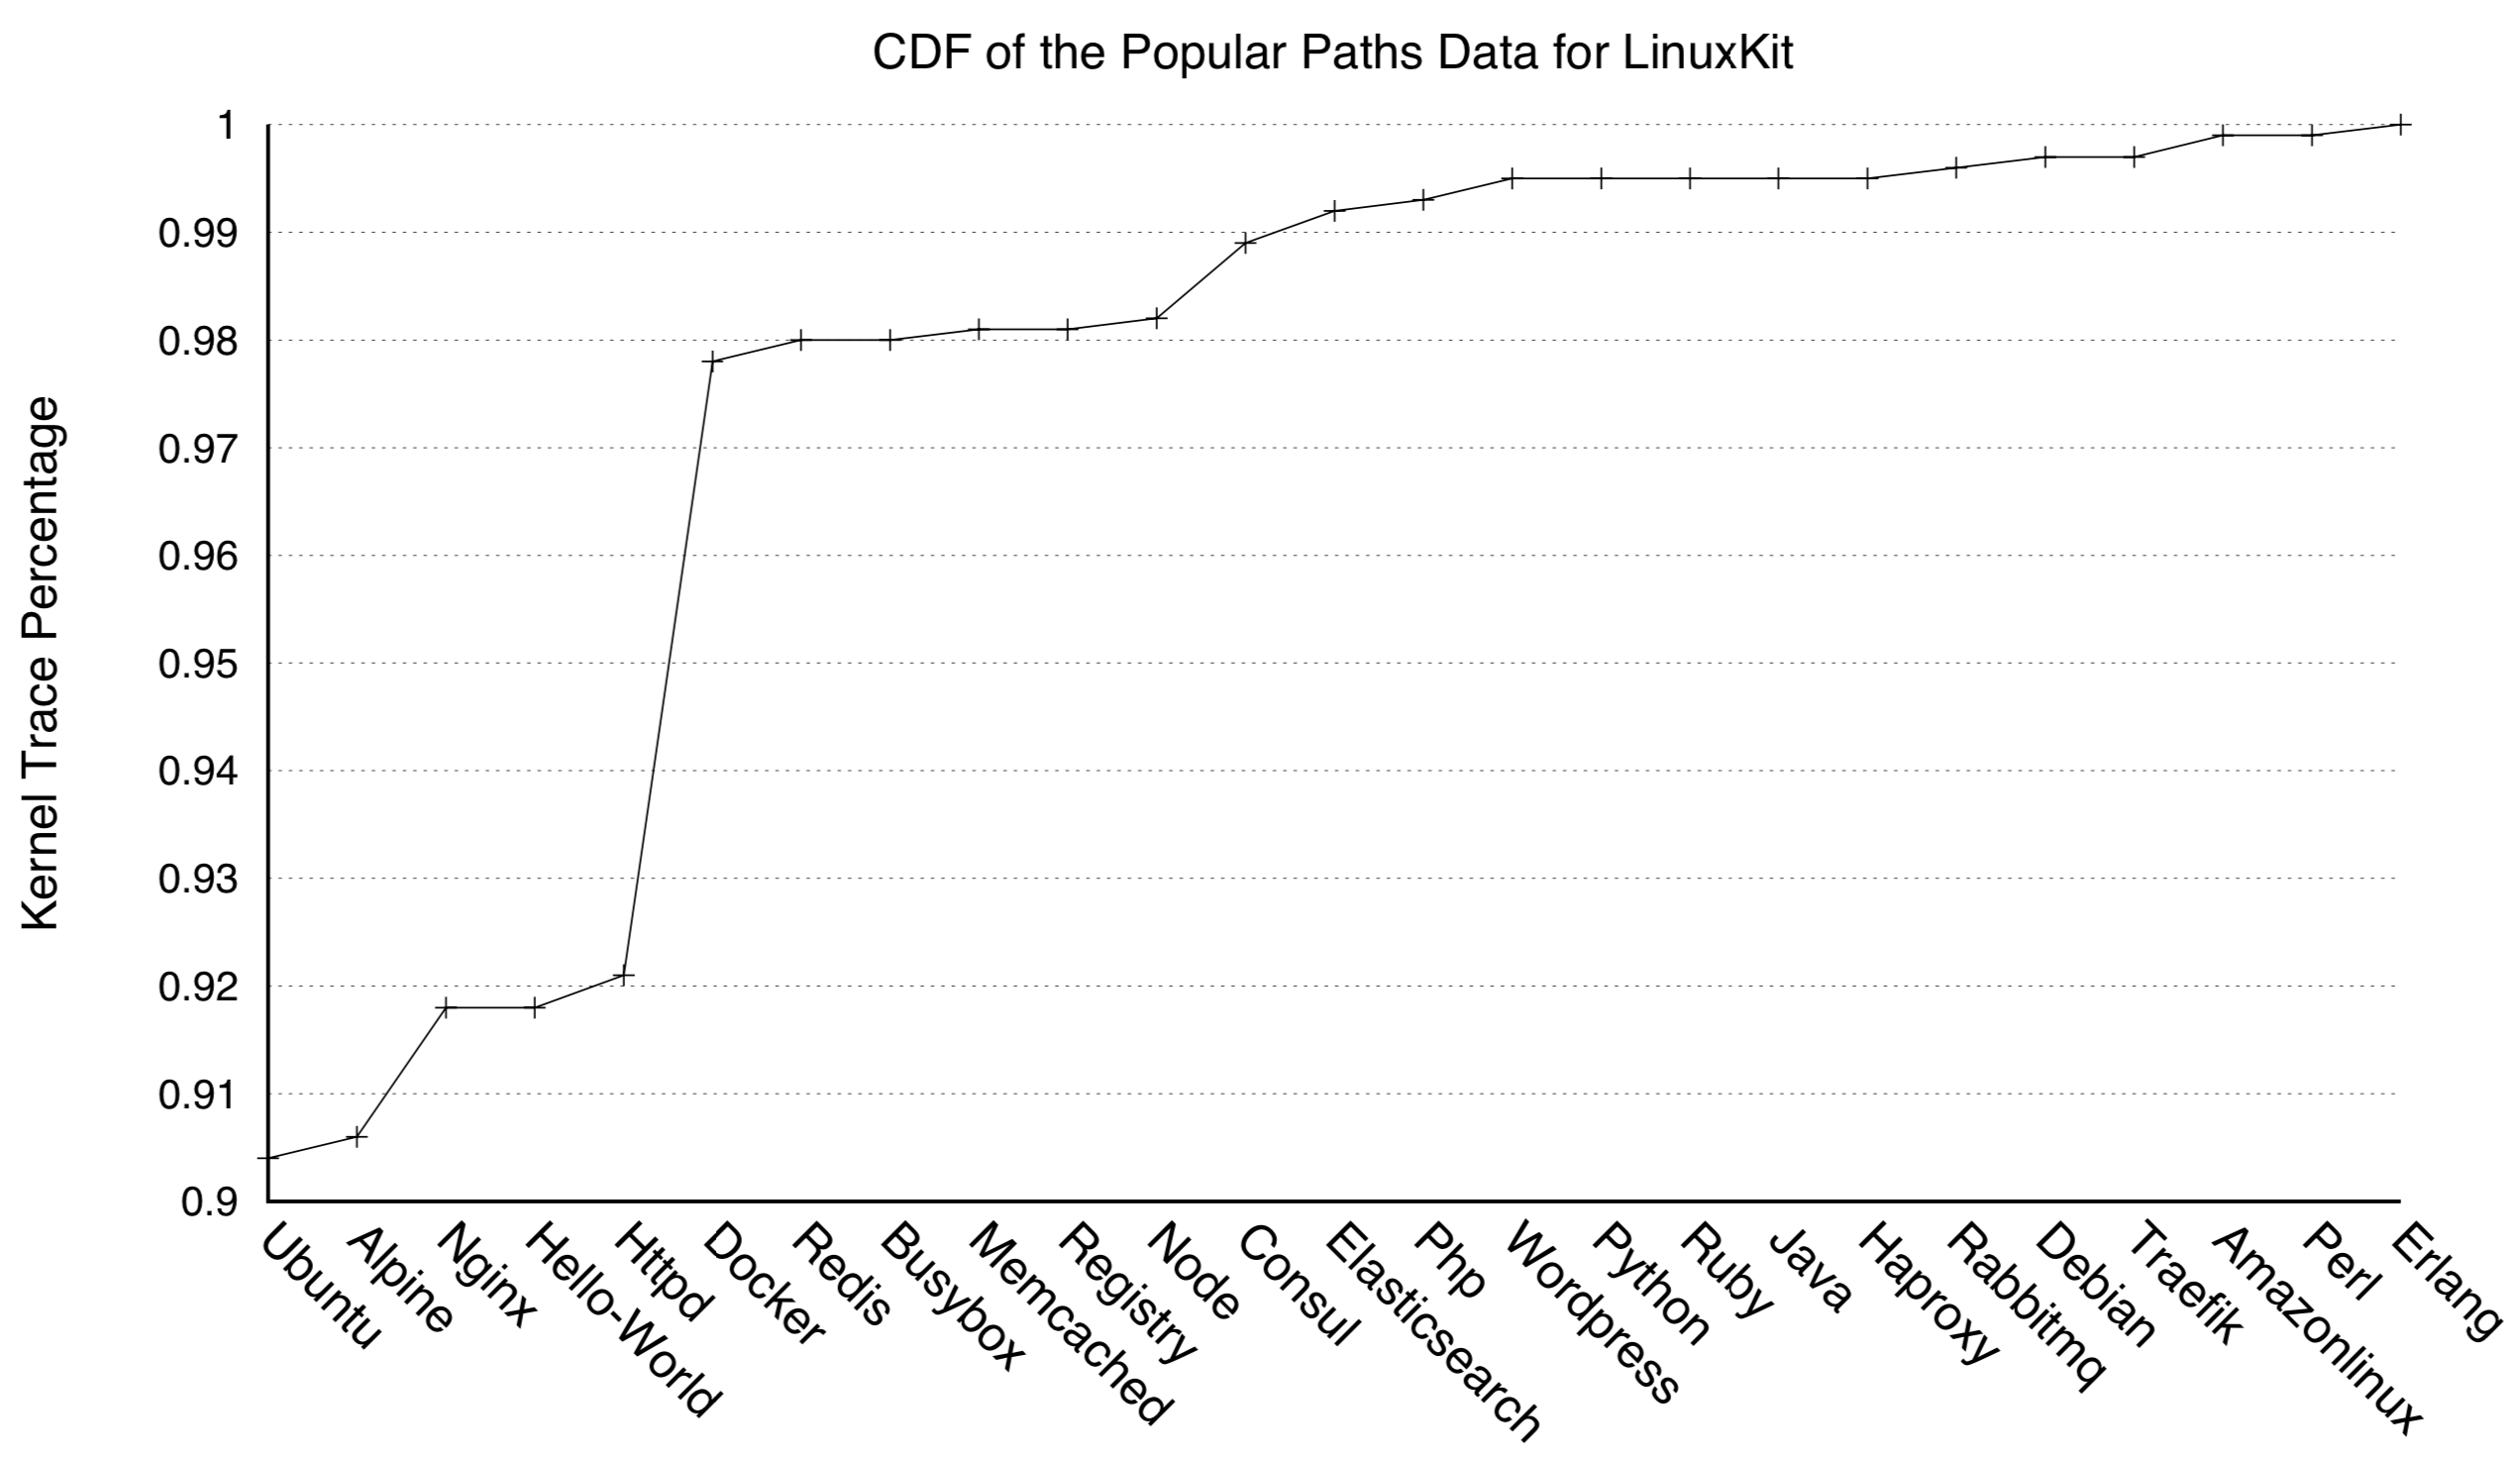
\includegraphics[width=1.5\columnwidth]{diagram/pp-cdf.png}
\caption{\small CDF of the popular paths of Docker containers showing most share the same kernel footprint}
\label{fig:pp-cdf}
\end{figure*}

In addition to the always used popular paths, which we identified as the common kernel lines that appeared each and every time, 
we also discovered certain lines of code that showed up sporadically. For these lines, we looked at what activities they performed, and how common they were across different containers. 
In our analysis of the kernel trace of 10 frequently used Docker containers, we identified eight pieces of infrequently executed kernel code common among them.  
These traces are presented graphically in Figure \ref{fig:cdf-marked}. 
\begin{enumerate}
	\item \verb|kernel/cgroup/freezer.c|: a cgroup is freezing if any FREEZING flags are set.
	\item \verb|kernel/locking/rwsem-xadd.c|: waiting for a write lock to be granted. 
	\item \verb|kernel/locking/rwsem-xadd.c|: waiting for the read lock to be granted.
	\item \verb|mm/filemap.c|: process waitqueue for pages and check for a page match to prevent potential waitqueue hash collision. 
	\item \verb|fs/exec.c|: all other threads have exited, wait for the thread group leader to become inactive and to assume its PID. 
	\item \verb|kernel/workqueue|: insert a barrier work in the queue. According to the comments from the kernel source code, 
	the reason for inserting a barrier work seems to be to prevent a cancellation. 
	This is because \\
	\verb|try_to_grab_pending()| can not determine whether the work to be grabbed is at the head of the queue and thus can not clear LINKED flag of the previous work. 
	There must be a valid next work after a work with a LINKED flag set. 
	\item \verb|arch/x86/kernel/tsc.c|: try to calibrate the TSC \\ 
	against the Programmable Interrupt Timer and return the frequency of the TSC in kHz. 
	\item \verb|kernel/locking/mutex.c|: hand off a mutex. Give up ownership to a specific task, when @task = NULL, this is equivalent to a regular unlock.
\end{enumerate}

\begin{figure*}
\centering
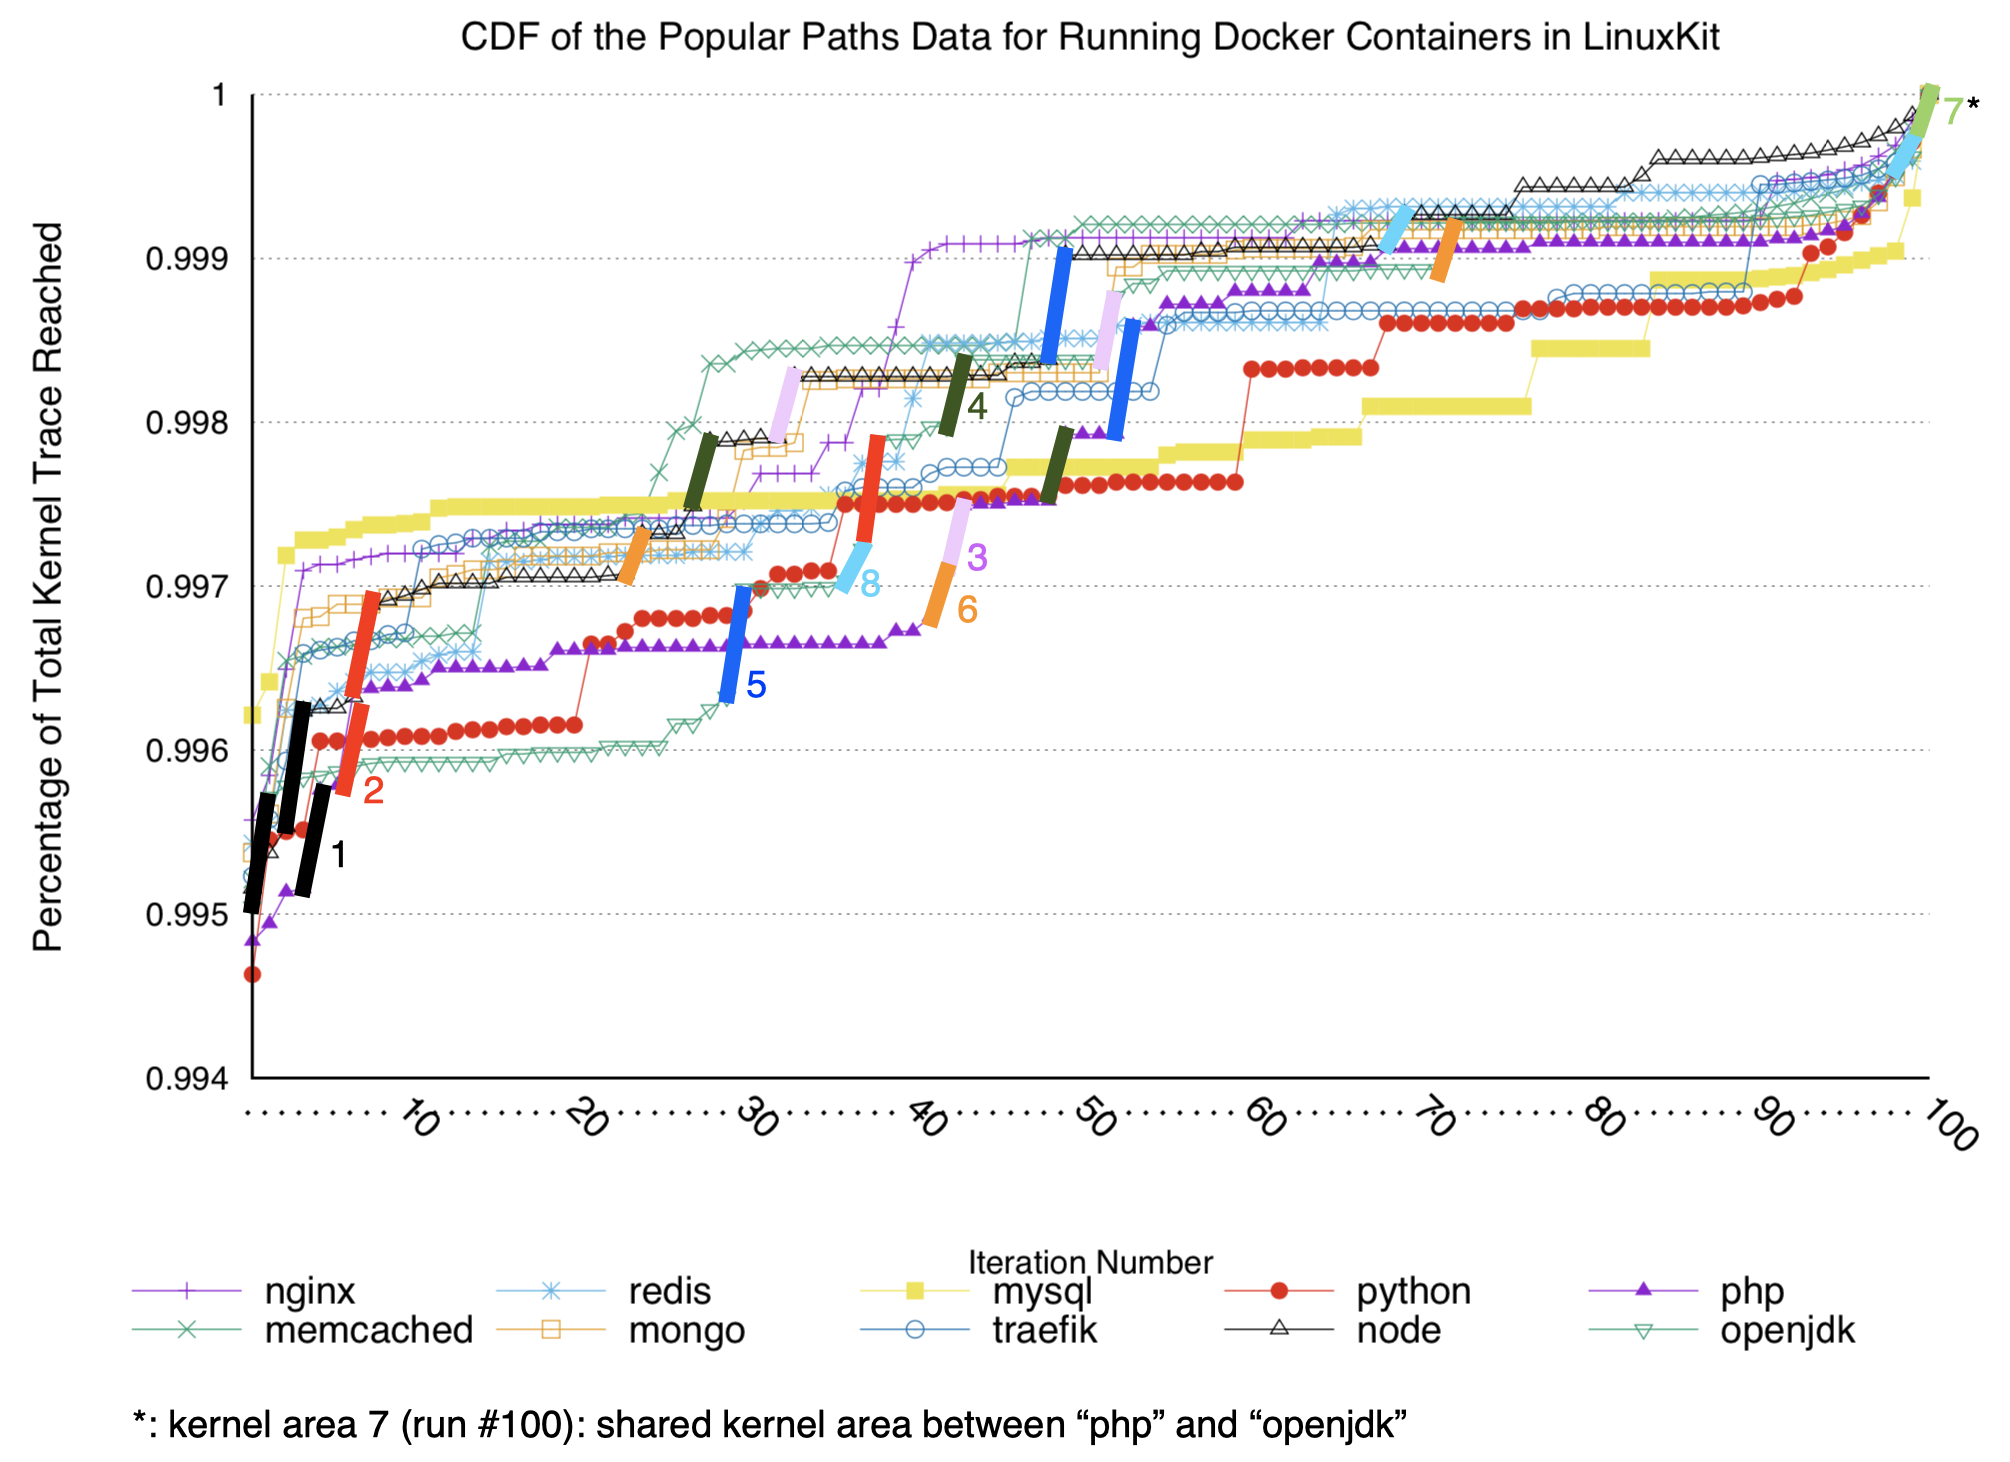
\includegraphics[width=1.5\columnwidth]{diagram/cdf-marked.png}
\caption{\small Common kernel code identified across different containers}
\label{fig:cdf-marked}
\end{figure*}

What this analysis tells us is that, despite the fact that they are infrequently executed, this  code performs essential kernel functions and is used by multiple containers. 
Therefore, we considered them popular paths, and included them in our popular paths kernel profile. On closer examination, we learn they are not always executed during each run  because, 
as largely race-condition related codes (except for code \#7), they depend on locks, and on system conditions that may vary during different runs. 
Being able to capture these examples of infrequently-executed code and include them into our popular paths profile is important, because it makes the UnPAK unpopular kernel logs more accurate, 
and therefore is key to aiding efficient security auditing. 


\subsection{Can real-world containers run on the UnPAK auditing kernel with no loss of functionality?}
\label{sec.evaluation.3} 
To demonstrate that the UnPAK kernel can support efficient auditing in practice, we needed to confirm that, as compared to the original Linux kernel, 
it will not break any essential kernel functionalities, and can support real-world containers.

To affirm this, we ran a set of tests, the first of which used the Linux Testing Project (LTP) \cite{LTP} test suites. 
We used this open source test project designed to validate the reliability, robustness, and stability of Linux to verify that UnPAK functions as anticipated. 
The second test involved running a collection of the most popular containers from Docker Hub to verify if they were able to function correctly if they ran on UnPAK auditing kernel.

\subsubsection{Testing functionality with the LTP test suites}
\label{sec.evaluation.3.1} 
\textbf{Experimental Setup:} We used the Dockerfile provided by LinuxKit \cite{LinuxKit} to create the container image that runs the LTP version 20170116. 
This test project offers a set of regression and conformance tests designed to let members of the open source community confirm behavior of the Linux kernel. 
The test script we ran consisted of 798 test cases that verified the correctness of system functionalities, such as memory allocation, network connection, file system access, locking, and more. 
Using the test suites, we ran our experiments inside of a LinuxKit version 0.2+ virtual machine. The machine was built using Docker version 18.03.0-ce running on 
a host operating system of Ubuntu 16.04 LTS, with Linux kernel 4.13.0-36-generic. A QEMU emulator version 2.5.0 served as the local hypervisor. 

\textbf{Results:}  UnPAK was able to run all of the 798 test cases, and produced the same results as the original Linux kernel. 
This indicates that our UnPAK audit kernel implementation, using KVM hypercalls, can provide correct functionality. 
Among all these tests, 673 of them generated ``success'' as their expected output on both kernels. We observed 105 test cases returned ``failures'' as expected, 
mainly because of restrictions imposed by LinuxKit. For example, ``mem01'' test failed because the malloc function failed to allocate 3056 MB memory due to the default memory restriction. 

\subsubsection{Testing functionality on real-world container applications}
\label{sec.evaluation.3.2} 
\textbf{Experimental Setup:} To confirm that UnPAK could run applications in real-world practice, we identified the 100 most downloaded containers from Docker Hub, 
and ran them in the same version of the LinuxKit virtual machine used in the test described in 4.3.1. Each container was run in the LinuxKit VM using the commands from its official Docker image. 
To take into account any potential variances, each container was run 10 times in the exact same environment. We used the top 50 popular containers as the training dataset to 
get the popular paths kernel profile, and then tested our UnPAK kernel with these 50 containers plus 50 other popular containers. 

\textbf{Results:}  We verified that the 100 containers run using UnPAK were able to finish their normal workloads with, on average, less than 1\% of runtime overhead. 
In doing so,  less than 0.1\% of the total kernel lines reached were unpopular. And these unpopular lines appeared both in the 50 containers used in the training dataset, 
as well as in the 50 new containers in the testing dataset. Using our list of 50 CVE bugs, we verified that these unpopular paths logged by UnPAK contained none of the bugs. 
(These unpopular lines were mostly rarely executed race-condition related code) 

The results show that real-world containers will not generate unpopular kernel logs in the overwhelmingly majority of (>99.9\%) cases. 
This is expected, since no malicious party or attackers were actually trying to exploit any vulnerabilities in our testing. 
It shows that our UnPAK kernel works as expected when auditing on popular real-world containers. 

\subsection{Performance Evaluation}
\label{sec.evaluation.4} 
\textbf{Running real-world containers with UnPAK}
\newline
Adoption of UnPAK is dependent on its real-world viability. So, the next round of tests were to ensure it would not negatively affect performance overhead costs. 
To demonstrate this, we evaluated both the run-time performance and memory space overhead of the UnPAK audit kernel.

\textbf{Experimental Setup:}
We compared data from containers running on the original Linux kernel and on the 
UnPAK kernel and measured the overhead costs. We used the exact same running environment and configuration to ensure a fair comparison. 
In each test, the container finished its workload as defined in the official Dockerfile. We then measured the runtimes for both kernels and compared them. 

\textbf{Results:} 
On average, the results show running containers on UnPAK incurred about 0.5\% to 1\% of extra performance overhead, as compared to the original kernel. 
Results of the top 10 containers are shown in Figure \ref{fig:performance}. (For each container, the runtime was the average runtime of 10 runs.)

\begin{figure}
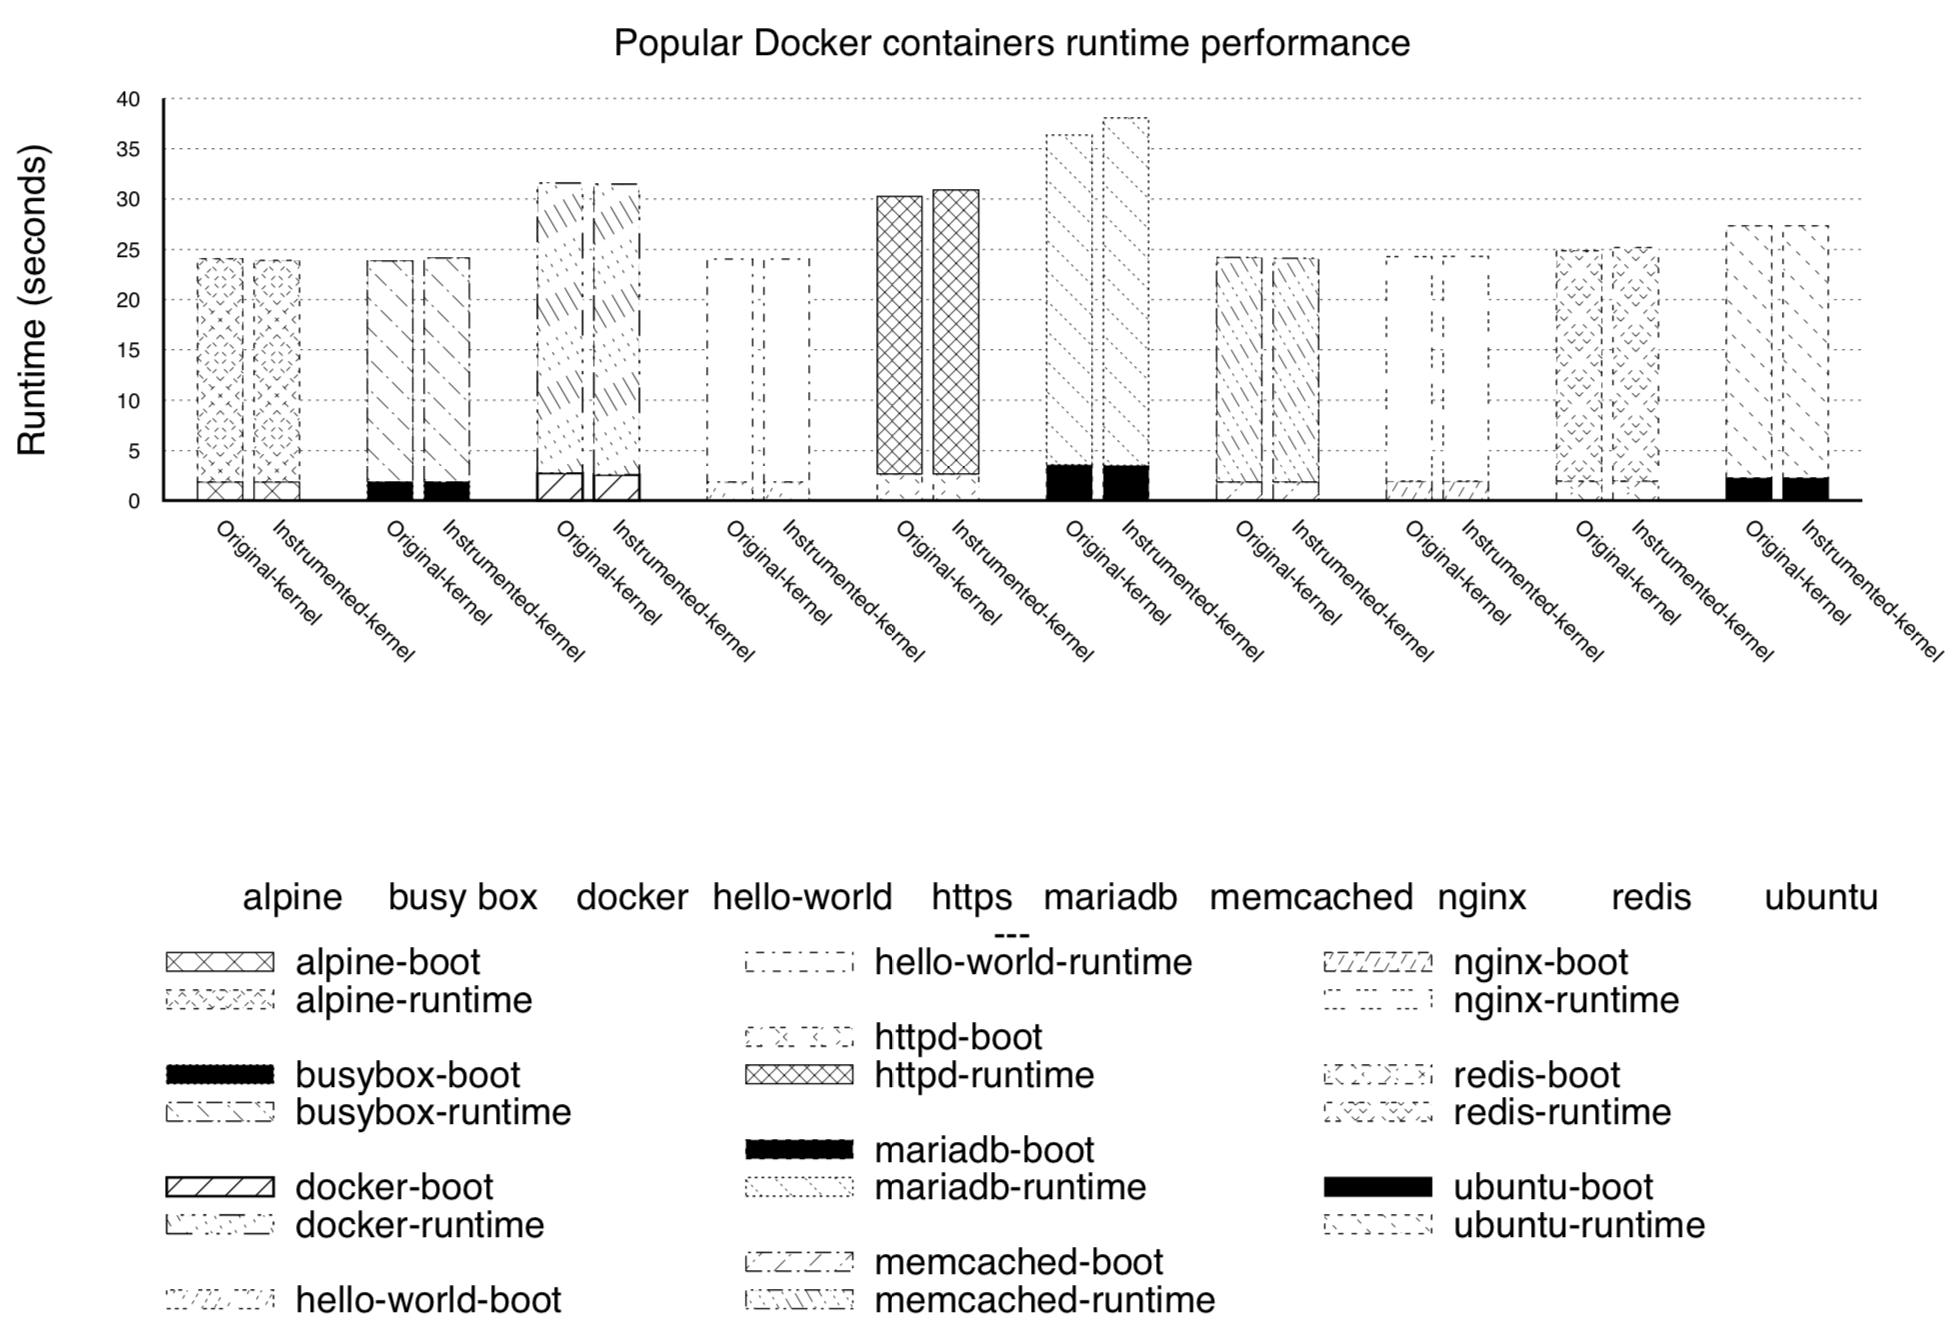
\includegraphics[width=1.0\columnwidth]{diagram/performance.png}
\caption{\small Runtime performance comparison for the top 10 containers}
\label{fig:performance}
\end{figure}

The original Linux kernel image used for the LinuxKit test  is sized at 163,012,008 bytes. In comparison, UnPAK is sized at 163,622,440 bytes. 
Thus the extra memory space added by our modified kernel was only about 0.37\%. 

In summary, for both runtime and memory space UnPAK has negligible overhead.

\subsection{Is forensic auditing using SmashPAK efficient?}
\label{sec.evaluation.5} 
Lastly, but most importantly, we needed to assess if our SmashPAK data structures could actually support  forensic auditing without any substantial drawbacks. 
To do so, we performed the  operations defined in Section 3, Step 3 on a collection of SmashPAK kernel data. 
The UnPAK kernel emits SmashPAKs at a specific frequency for each container and each one will have a small set of potential time periods.  
As the SmashPAKs from relevant containers are collected and combined into the overall collection, the total scope and span will grow. 

For each released kernel, there is a fixed amount of basic blocks for the kernel codebase. So each SmashPAK has a fixed length of indices. 
For the kernel we implemented, there is a total number of 158,929 unpopular basic blocks, so we have 158,929 indices for our SmashPAK. 
Each index points to a list of occurrences. The occurrences data structure has a maximum fixed size, so the total size of each SmashPAK is fixed and relatively small. 
For example, we set the maximum size of our occurrences list to 10, and use ``int'' (four bytes) to store the information. 
The total size of each SmashPAK is only around 10 mb, and considering that many SmashPAKs could be combined, 
modern machines or cloud services conducting security audits could easily store millions. 

We implemented SmashPAK with our kernel size (158929 unpopular basic blocks). 
The average time cost of a search operation for a CVE bug in SmashPAK was 0.1598 seconds. 
The average time cost of a combine operation for two SmashPAKs was 0.2422 seconds for almost empty (<=10\% filled) occurrences lists, 
and 0.8399 seconds for almost full (>=90\% filled) occurrences lists. 

Considering that the end user who conducts the audit is likely a human being, such as system administrator, 
committing only about 0.16 seconds searching to learn if (and when) a CVE  could have been triggered at a particular location for a container is very efficient in practice.
%\section{Limitations}
\label{sec.limitation}
While our results and analysis indicate that our dataset was representative of the workload container applications perform, the sample size was somewhat limited and therefore, 
so was the amount of data gathered. Additional runs and a larger sample base could potentially capture the race-condition related kernel footprint more comprehensively, 
thus rendering more accurate data. 

Another factor that could have affected our results was the type of images we used. We limited our selection to official container images from Docker Hub, 
yet there are a number of open source project images we did not access. If we had run these additional images using the same methodology, 
it might have yielded a broader spectrum of results.

Our implementation is currently focused only on warning users whenever there is a potentially dangerous attempt to trigger an unpopular line of code. 
There are certainly more ways we could have explored to deal with risky attempts to reach unpopular lines. 
For example, we could have instrumented the kernel to try to exit the VM and block the container from executing more code to avoid any further security breach. 
Another possible strategy is to first monitor any attempt to access the unpopular lines, and then dynamically remove the unpopular code binary from the memory at runtime 
to prevent potential exploitation of bugs. We leave evaluation of these options as future work.

Lastly, all the research documented in this paper was conducted only with Linux kernel version 4.14.24. 
For future work, we plan to extend our system so that it can automatically work with other kernel versions. 
This will generalize the application of our work, and potentially help a lot more users secure their containers. 
\section{Related Work}
\label{sec.related_work}
In this paper, we seek to enhance the security of containers running on top of the host kernel by reducing exposure to the rarely-used risky code in the kernel. 
When developing our strategy, we consulted previous studies in three areas: 
1) metrics for vulnerability prediction, 2) techniques for enhancing kernel security, and 3) approaches for enhancing container security. 

\textbf{Estimating and predicting vulnerabilities.} 

Metrics that can identify code most likely to contain vulnerabilities help developers and researchers prioritize their efforts to fix bugs and improve security. 
Chou et al. \cite{Chou} looked at error rates in different parts of the operating system kernel, and found that device drivers had error rates up to seven times higher than the rest of the kernel. 
Ozment and Schechter \cite{Ozment} examined the age of code as a predictor of vulnerability in the OpenBSD \cite{OpenBSD} operating system, 
and generally confirmed the finding that the rate at which bugs are found goes down over time. 
In a recent prior work \cite{Lock-in-Pop}, Li et al. directly compared both of these metrics to the  popular paths metric, and found that neither was as predictive of vulnerabilities in the Linux kernel.

Shin et al. \cite{Shin:2011:ECC} examined code churn, complexity, and developer activity metrics, 
finding that these metrics together could identify around 70\% of known vulnerabilities in the two large open source projects codebase they studied. 
However, file granularity is too coarse to be useful when deciding which parts of the kernel need protection. 
Customizing the operating system kernel to work at the lines-of-code level, as the popular paths metric does, can be more effective. 

\textbf{Operating System kernel security enhancement.} 

Prior research in enhancing kernel security requires refactoring or modifying the kernel. 
Engler et al. \cite{Engler:1995:EOS:224056.224076} introduced the Exokernel architecture, which allowed applications to directly manage hardware resources in the hope of gaining efficiency in accessing the hardware. 
This style of operating system design came to be known as a library OS. More recently, but in a similar spirit, unikernels, 
such as Mirage \cite{Madhavapeddy:2013:ULO:2451116.2451167} run each application as its own operating system inside of a virtual machine, customizing the ``kernel'' for each application. 
Each of these systems, however, requires significant changes to existing applications (e.g., in the case of Mirage, applications must be rewritten in the OCaml programming language \cite{OCaml}.) 
Other library OSes are written to run existing applications. Drawbridge \cite{Porter:2011:RLO:1950365.1950399} and Graphene \cite{Tsai:2014:CSI:2592798.2592812} support unmodified Windows and Linux applications, 
respectively, by implementing an OS ``personality'' as a support library in each address space to improve security. 
However, user-space reimplementation of OS functionality incurs a performance overhead. Containers can mostly avoid this overhead, since they allow contained applications to make system calls directly. 
Thus, our work focused on the container-based approach. 

\textbf{Container security enhancement.} 

Existing security mechanisms available for containers usually leverage host kernel features. Namespaces \cite{namespaces} is one mechanism that can provide isolation between processes, and has been adopted by Docker. 
Linux capabilities \cite{linux-kernel-capabilities} allow users to define and choose smaller groups of root privileges, and thus can reduce the number of entities that can exploit  containers. 
Docker containers use Linux capabilities, and LinuxKit allows users to define and control the capabilities (such as file permissions) they want to use. 
While these existing approaches do help improve security for containers, they also have limitations. First, it can be really hard to understand how to correctly configure the security settings for containers. 
In fact, many users just use the default configuration, which may not be the best choice if strong security is needed. 
Second, in order to run the applications a user wants, containers still need  to allow access to risky code in the host kernel. 
Our work improves the container security by imposing a fine-grained security monitor and control over access to the potentially risky kernel code.
\section{Conclusion}
\label{sec.conclusion}
In earlier work, we found that running applications using only frequently used popular paths could improve the security of virtual machines. 
As a follow-up we wanted to test the feasibility of applying this popular paths metric to existing containers. 
To do so, we developed a methodology to systematically profile and obtain the popular paths data of widely-used container applications. 
Using this data, we were not only able to create UnPAK, a modified Linux kernel that could alert users whenever potentially dangerous unpopular lines are about to be triggered, 
but  also identify ways to improve security at various levels of granularity. By allowing users to improve container security with steps as simple as eliminating unused files, 
it means that those who can not do the more labor intensive work of eliminating bugs at the line of code level do not need to remain completely vulnerable. 
Security thus stops being an ``all or nothing'' proposition, but instead can be tailored to the security sensitivity of the application and the available resources of the user. 

We were also able to verify that, consistent with previous findings, the popular paths in the host kernel for frequently used Docker containers do contain fewer security vulnerabilities, 
and thus are inherently more secure. Equally important, usingUnPAK, we were able to prove that  these containers were able to run their default workload using the popular paths 
more than 99.9\% of the time, with only a negligible (less than 1\%) performance overhead based on its current action configuration. 
Compared with three other current kernel tailoring strategies, we demonstrate that UnPAK was an efficient solution in reducing the kernel attack surface, with relatively fewer limitations. 

%
% The next two lines define the bibliography style to be used, and the bibliography file.
\bibliographystyle{ACM-Reference-Format}
\bibliography{paper}
\end{document}